\section{Pipeless plant} %

In chemical industry, pipeless plants are used due to its high flexibility level. In these type of plants, Automated Guided Vehicles(AGVs) are used to transport the vessel from one processing station to another. Thus, for each and every batch, the AGV transport the vessel to various stations to create an end product, making the pipeless plant multi-product and multipurpose chemical production. In this way, piping and the associated cleaning is eliminated, thus aiding in cost and energy efficiency.

\subsection{Experimental pipeless production plant}
 
 The pipeless plant framework in the TU Dortmund, developed by the Process Dynamics and Operations Group (DYN), consists of four AGVs, two color stations, one mixing station and one storage station. Each station has a role in producing batch of plaster art, for example mixing or filling the product in the vessel. The stations and the AGVs are controlled by a Programmable Logic Controller(PLC). The vessel on the AGV is moved from one station to another based on the schedule to produce a batch. Regarding the positioning system, the plant uses a camera to identify the LED pattern on the AGV. Each AGV has a unique pattern that distinguishes it from another.


\begin{figure}[!htbp]
	\centering
	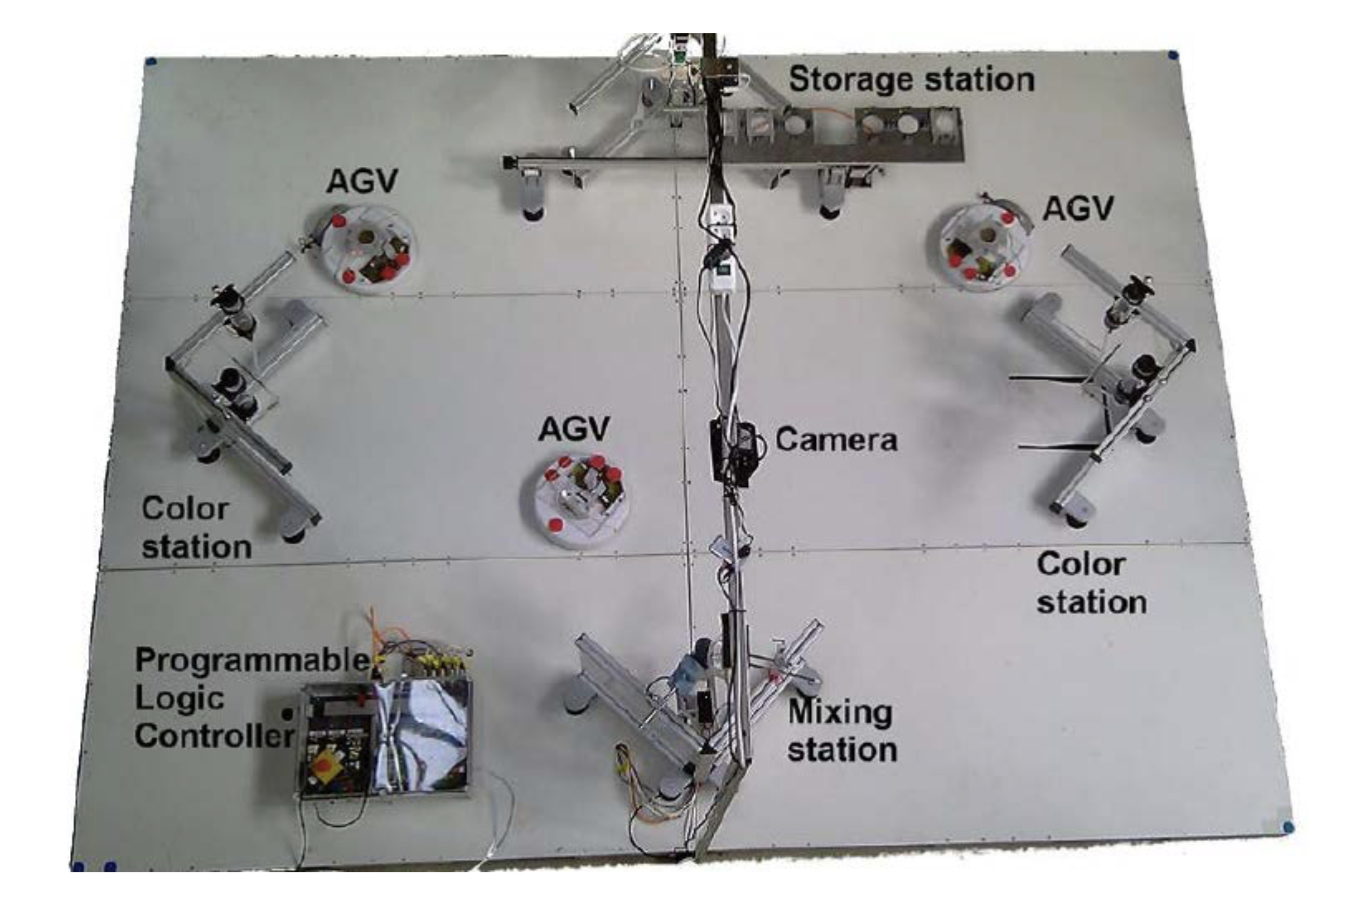
\includegraphics[width=14cm]{Pictures/Plant.png}
	\caption{Existing setup}
	\label{Pipeless plant}
\end{figure}


\subsection{Problems with the existing setup}

Since the existing setup uses vision based positioning system, the plant suffers various disadvantages as described below:
\begin{itemize}
\item During bright day-light conditions, no position is updated by the camera. This is due to the fact that the threshold of the sunlight and the LED on the AGV becomes equal that the camera fails to detect any pattern, thus affecting the whole system efficiency.
\item The camera suffers the so called fish-eye camera lense problem, meaning that the position error is proportional to  distance from the center of the image. This is caused by the distortion a wide angle lens.
\item The restriction of usage of incoming information from the camera during software implementation.
\item The percentage error and the processing time increases with the increase in number of robots to be localized thus affecting the controller input.
\end{itemize}


All these cons added up together cause a deterioration in the accuracy of the position of the AGV, which in turn affects the controller leading to a drop in system efficiency. 

\subsection{Project objectives}

The disadvantages of the vision based positioning systems as discussed above leads to the urge for creating a localization that overcomes all the cons already suffered.\\

This projects aims to research about alternative positioning system and to evaluate with the selected technique by simulation. The ultimate goal is to develop a positioning system with  improved position precision and to compare and develop practical proof-of-concept.

